\section{Rapport de fin d'itération}

Le développement de l'itération 1 s'est bien déroulé. La charge de travail a 
été correctement répartie le long des 3 semaines de développement, tout le monde
a pris part de manière équilibrée au travail et on ne déplore aucun conflit.\\

\subsection{Suivi du planning}

Toutes les sous-histoires de l'itération 1 ont été implémentées et nous estimons
avoir réussi à le faire tout en gardant une architecture propre.\\

Le temps étant court et la fonctionnalité demandée étant plutôt grande, nous 
avons d'abord commencé en petits groupes pour la découverte des outils et
librairires que nous allions utiliser. Nous avons ensuite essayé de tout mettre
ensemble pour tester le produit complet à un stade pré-alpha.\\

C'est à ce moment que nous avons effectué un premier refactoring pour pouvoir
tous continuer sur les différents aspects du projet dans une architecture propre.

	\subsubsection{Timesheet}
	\resizebox{\linewidth}{!}{
	\begin{tabular}{l|c|c|c|c|c|c}
		\textbf{Tâche} & \textbf{Bruno} & \textbf{Florentin} & 
		\textbf{Julian} & \textbf{Pierre} & \textbf{Titou} & \textbf{Walter}\\ \hline
		Management&6,00&19,00&6,00&6,00&6,11&6,00\\ \hline
		Découverte lib 3D&7,00&5,75&&&&\\ \hline
		Compilation projet Eclipse/Ant&&&1,00&1,00&5,75&\\ \hline
		Découverte GUI (swing)&&&5,00&8,33&&1,00\\ \hline
		Model / Découverte ORMlite&&&&&4,00&\\ \hline
		Refactoring/Debug&&8,00&&11&3,00&\\ \hline
		1.1 Enregistrement d'un projet&&&&&18,00&\\ \hline
		1.2 GUI&6,33&&4,00&25,83&5,00&4,00\\ \hline
		1.3 Affichage du monde 2D/3D&15,00&11,00&9,00&&2,00&12,00\\ \hline
		1.4 Navigation dans le monde 3D&12,00&&&&&2,00\\ \hline
		1.5 Modif. de la géométrie des pièces&&8,00&&&6,00&12,00\\ \hline
		1.6 Création d'un demo project&&&&&&\\ \hline
		1.7 Enregistrement automatique &&&&3&2,00&\\ \hline
		1.8 Intégration GUI+3D&4,00&2,00&3,00&1,00&5,00&\\ 
	\end{tabular}}

\subsection{Architecture}

	\subsubsection{Architecture générale}
	\begin{figure}
		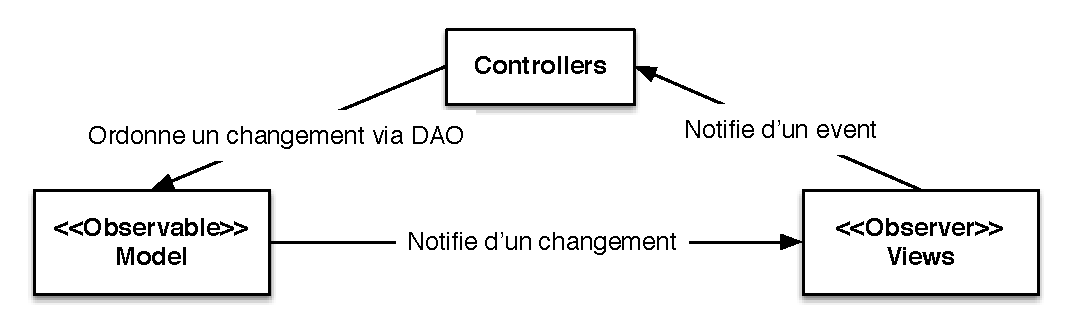
\includegraphics[width=\textwidth]{uml/general-architecture.pdf}
		\caption{\label{fig:mvc:components} Diagramme de composants général}
	\end{figure}

	On voit directement l'utilisation du MVC, couplé avec un design pattern
	Observable et un DAO. Cette architecture nous permet de :
	\begin{itemize}
		\item rajouter/supprimer une vue (+ contrôleur) très facilement
		\item garder toutes les vues à jour
		\item découpler un maximum toutes les parties de l'application
		\item garder l'état du projet entre deux sessions d'utilisation
	\end{itemize}

	Prenons un exemple : le passage d'une vue 3D à une vue 2D et inversement.
	Ce passage a des implications dans plusieurs vues. La première est
	bien évidemment l'éditeur général, qui doit afficher le monde différemment
	en fonction du mode; la deuxième est la toolsbar, qui permet de changer de
	mode.\\

	Quand on clique sur le bouton 2D/3D, la ToolsBarView notifie son contrôleur
	d'un event reçu. Le contrôleur utilise alors le DAO pour enregistrer que
	le mode a été changé. Le modèle a en effet une valeur de configuration qui
	stocke le mode. Ce dernier notifie alors toutes les vues concernées du 
	changement (via le pattern Observer), dont l'éditeur principal qui va alors
	changer son mode d'affichage.\\

	\begin{figure}
		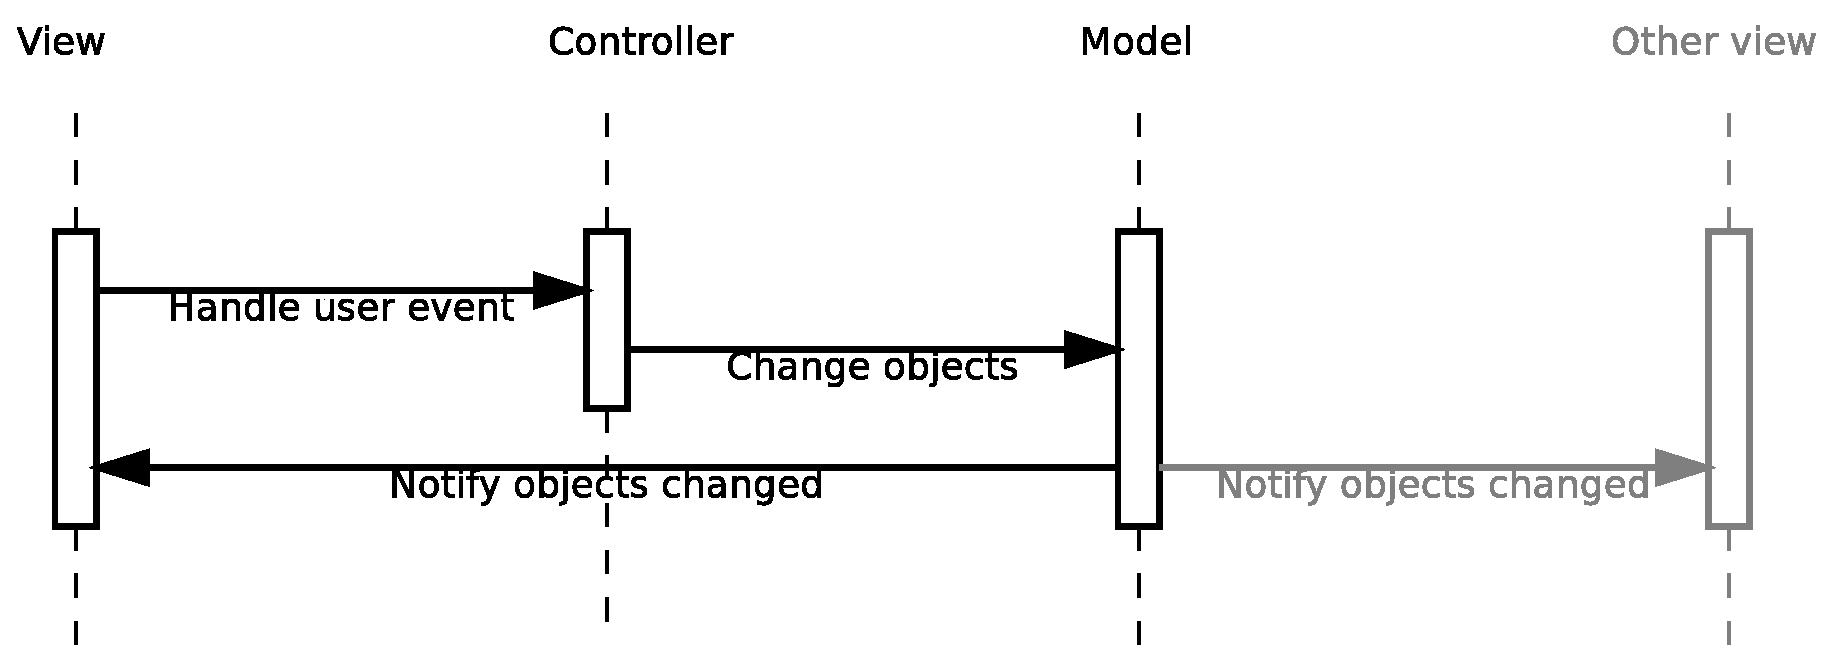
\includegraphics[width=\textwidth]{uml/MVC-sequence.eps}
		\caption{\label{fig:mvc:sequence} Diagramme de séquence MVC}
	\end{figure}

	\subsubsection{Architecture du modèle}
	Le modèle est architecturé selon le design pattern Data Access Object.
	La classe \texttt{Project} a la responsabilité de l'accès au fichier du
	projet, et des valeurs de configurations générales. Il donne en outre accès
	au \texttt{GeometryDAO}, qui est un singleton pour le projet, et qui permet
	d'effectuer les opérations CRUD\footnote{Create Refresh Update Delete},
	ainsi que des recherches d'objets selon différents critères.

	Les objets enregistrables par le \texttt{GeometryDAO} implémentent tous
	l'interface \texttt{Geometric}. On distingue 4 catégories d'objet dans le
	modèle (Figure \ref{fig:models:classdiagram}):

	\begin{itemize}
		\item Les \texttt{Point} représentent une position dans l'espace
		\item Les \texttt{Shape} définissent des formes bidimensionnelles 
		      composées de \texttt{Point}
		\item Les \texttt{Grouped} définissent des constructions sur les 
		      \texttt{Shape}
		\item Les \texttt{Floor} permettent de grouper ces éléments par étage.
	\end{itemize}

	La séparation de la forme et des constructions nous permet d'associer
	facilement différents éléments de la pièce (murs, sols, plafonds) qui sont
	bâtis à partir des mêmes points. En outre, plusieurs pièces peuvent contenir
	le même point, facilitant ainsi la détection de pièces adjacentes, le
	déplacement d'un coin de mur entre plusieurs pièces, ...

	\begin{figure}
		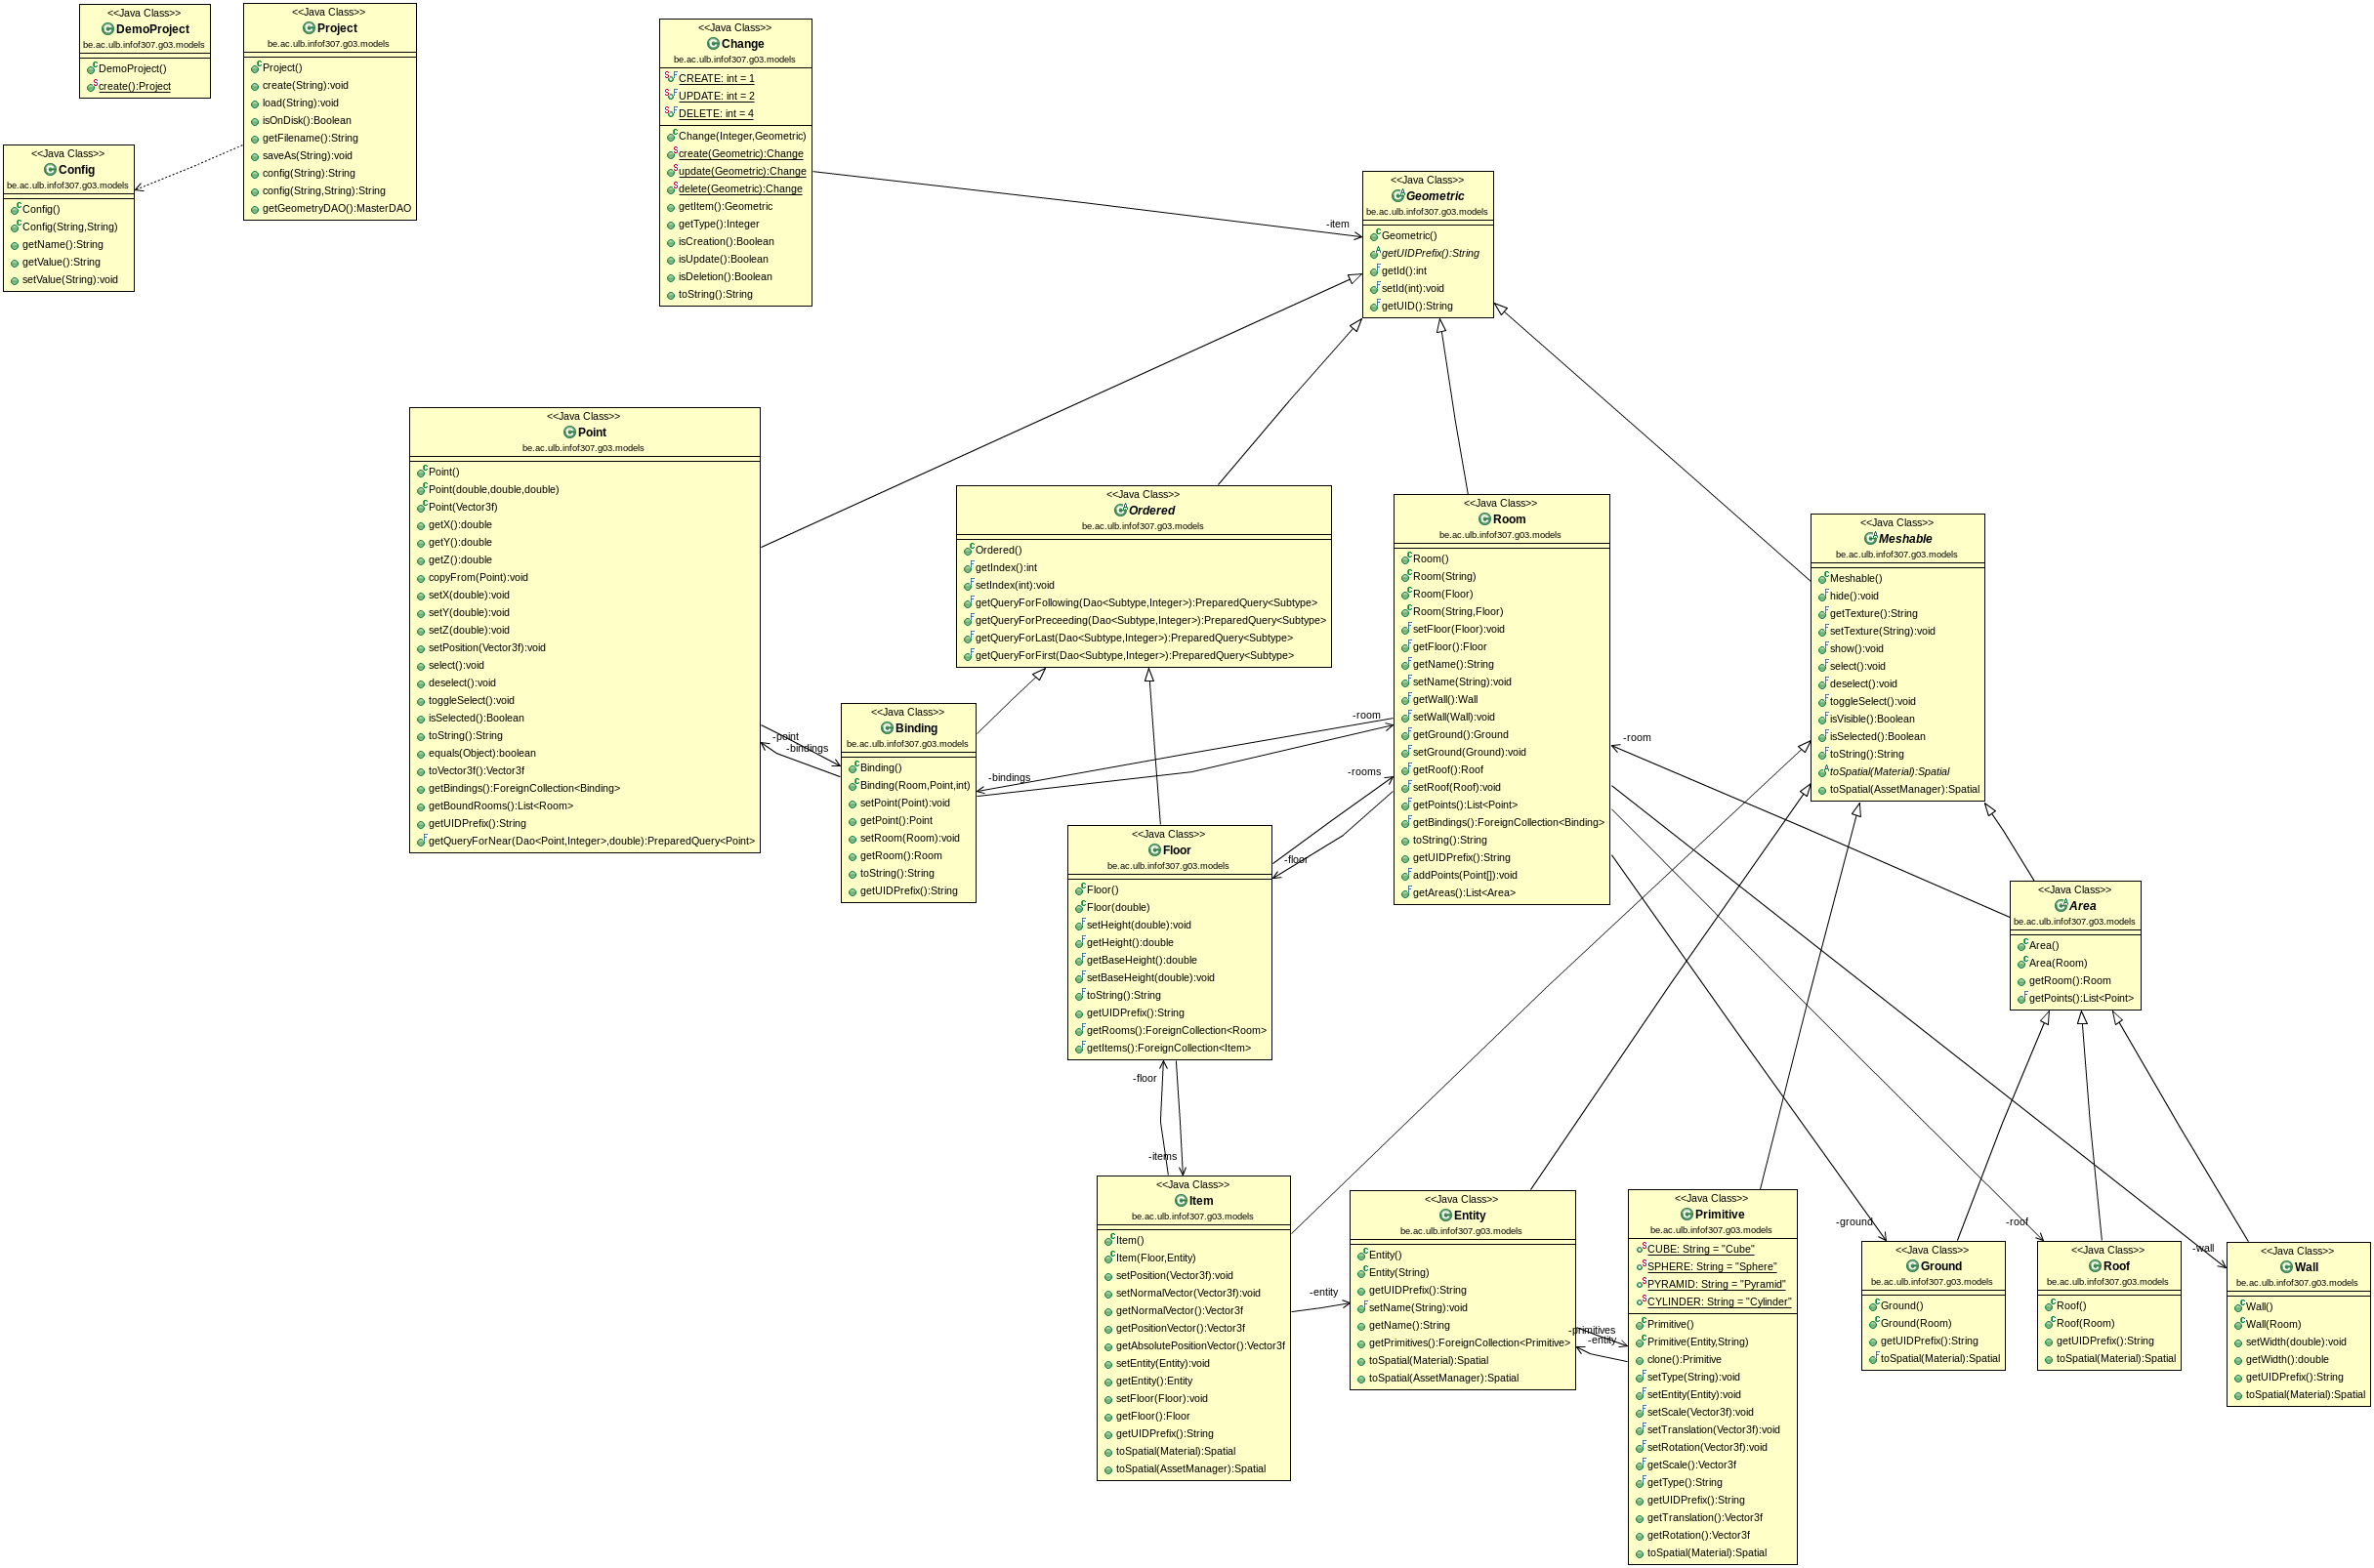
\includegraphics[width=\textwidth]{uml/models.png}
		\caption{\label{fig:models:classdiagram} Diagramme de classes du modèle}
	\end{figure}

	\subsubsection{Architecture de la GUI}

	L'interface graphique est composée de plusieurs vues qui ont chacune leur 
	contrôleur propre. La classe GUI est celle qui gère la fenêtre et les 
	composantes de premier niveau : 
	\begin{itemize}
		\item la barre de menus
		\item les popup de sélection de fichiers
		\item la barre d'outils
		\item l'éditeur principal (qui gère la vue 3D/2D et la TreeView)
	\end{itemize}

	La WorldView est une sous-classe d'une SimpleApplication jMonkey. C'est
	le canevas 3D à proprement parler. 

	\begin{figure}
		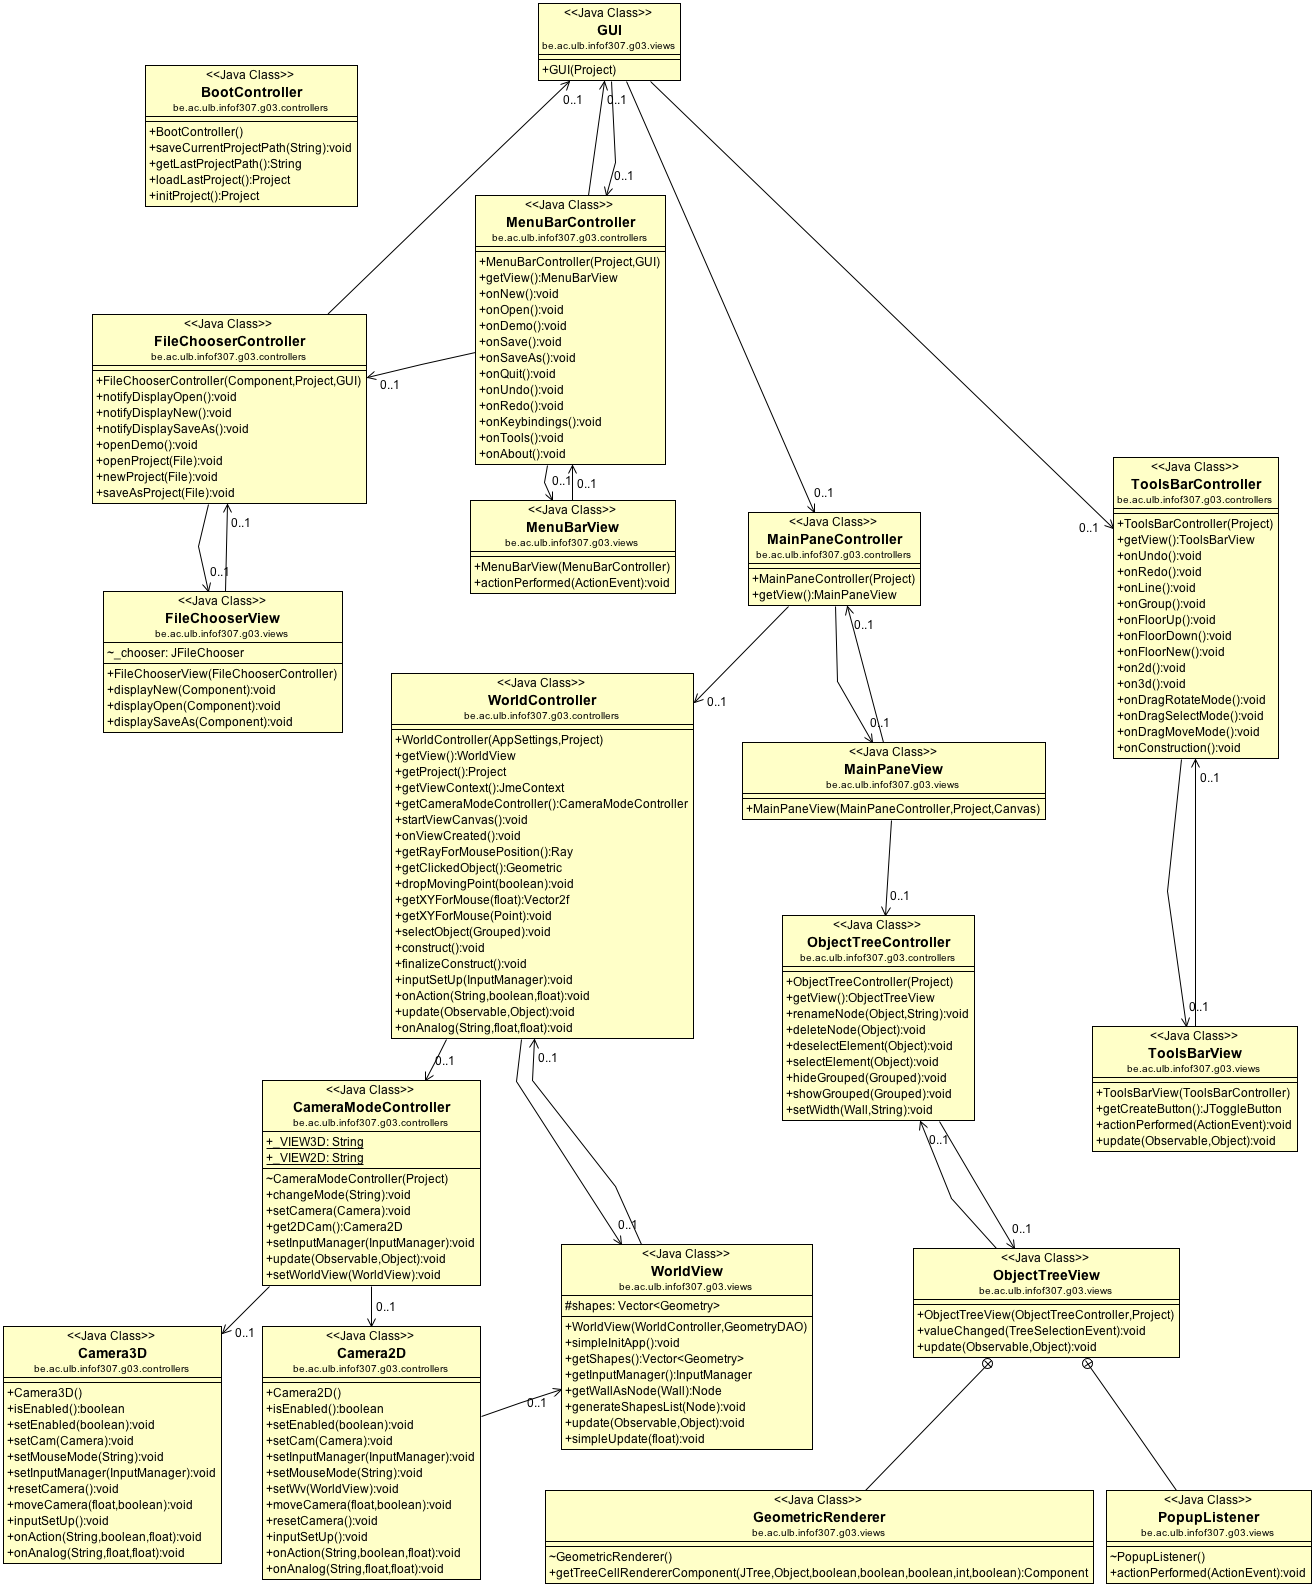
\includegraphics[width=\textwidth]{uml/gui.png}
		\caption{\label{fig:GUI:classdiagram} Diagramme de classes de la GUI}
	\end{figure}

\subsection{Bonnes pratiques utilisées}
Plusieurs pratiques ont été mises en place pour faciliter le développement en 
groupe, comme par exemple le pair programming ou les sprints d'une journée.

	\subsubsection{Pair programming}
	\`A plusieurs moments, nous avons travaillé par deux sur un même ordinateur pour
	les problèmes plus épineux. Un développeur écrivait du code, et l'autre essayait
	de le corriger et de penser aux edge cases en même temps. Cela nous a permis de 
	partager beaucoup plus facilement des idées et de compléter des features
	complexes de manière rapide et robuste.

	\subsubsection{Sprints d'une journée}
	En déployant un outil de statistiques de notre repository Git, on voit que le 
	samedi est le jour de la semaine où l'équipe commite le plus. La raison de ce 
	pic est simple : à deux reprises lors de cette itération, nous nous sommes
	retrouvés ensemble physiquement, autour d'une grande table, pour travailler sur
	le projet. \\

	Au début de la matinée, nous faisions une réunion pour établir les
	objectifs de la journée puis nous nous lancions tous sur la production de
	features. C'est lors de ces sprints que l'avancement était le plus marqué et 
	que nous pouvions prendre du recul facilement sur ce qui avait déjà été fait, 
	et ce qu'il restait à faire.

	\subsubsection{Développement itératif/fractal}
	Cette pratique a été adoptée dès le début, mais nous nous sommes rendus compte
	vers la moitié de l'itération que nous l'utilisions mal. Le principe de cette
	technique est de considérer chaque feature comme une unité qu'on peut développer
	à plusieurs niveaux de \textit{perfection}. \\

	Nous nous sommes forcés de produire très vite des proofs of concept, ou 
	Minimum Viable Products pour les unités à développer. Cette unité était 
	alors souvent à un stade de fonctionnalité très pauvre, dont l'architecture 
	n'était pas forcément bien pensée. Il fallait alors réécrire, rajouter ou 
	déplacer du code pour améliorer le point de vue utilité autant que le point 
	de vue de beauté interne du code, afin d'arriver à une unité fonctionnelle 
	complète et qui s'intégrait bien dans l'architecture de l'application. \\

	Toutefois, lors de la première moitié de la première itération, nous sommes
	souvent tombés dans le piège du "\textit{perfectionnement d'abord}", en
	passant beaucoup de temps sur le perfectionnement utilitaire de l'unité.
	Nous aurions dû passer plus vite - une fois que l'architecture d'une unité
	était bien intégrée dans l'application - au développement des autres unités.

	\subsubsection{Test-Driven Development}
	Cette technique, qu'il ne faut plus expliquer, a été utilisée, surtout pour
	le développement du modèle et s'est effectivement avérée positive lorsqu'il
	a fallu se baser sur un modèle robuste.

	\subsubsection{Staging area}
	Nous avons créé une branche \texttt{stage} sur laquelle nous testions la 
	version de développement la plus récente de l'application. De manière
	régulière, nous passions tous les changements de \texttt{stage} en
	production sur \texttt{master}. La condition de mise en production était 
	simple : tout le code doit être documenté, et tout ce qui peut être testé
	doit être testé.

	\subsubsection{Couverture de la qualité du code}
	Des outils d'évaluation de la qualité du code ont été utilisés. Parmi eux, 
	on peut en noter trois : 

	\paragraph{EclEMMA}
	Cet outil nous a permis d'évaluer facilement la couverture des tests dans 
	l'application et nous permet d'estimer visuellement très rapidement cette 
	dernière.

	\paragraph{Missing Javadoc (Eclipse)}
	On peut configurer Eclipse pour afficher des warnings là où le code n'est
	pas documenté, ce qui est très pratique.

	\paragraph{PMD}
	Plusieurs d'entre nous ont installé PMD en fin d'itération pour évaluer le
	respect des conventions de code. Nous n'avons cependant pas pris le temps
	de "réparer" les quelques erreurs mises en évidence.

	\subsubsection{Continuous integration}
	Nous avons choisi d'utiliser Travis CI\footnote{\url{http://travis-ci.org}}
	pour tester tous les commits pushés sur le dépôt, et ainsi assurer
	l'intégrité de la compilation et des tests, et d'être notifiés des erreurs
	éventuelles. Ant\footnote{\url{http://ant.apache.org/}} nous permet de
	compiler le projet hors d'Eclipse.

	\subsubsection{Réunions hebdomadaires}
	Nous avons réussi à tenir notre objectif d'une réunion hebdomadaire. Le 
	bilan de ces réunions est positif; elles nous aidaient à prendre du 
	recul sur notre progression et à remettre tout au clair. 

\subsection{Réflexion sur les librairies choisies}

	Généralement, nous sommes satisfaits de nos choix.

	\subsubsection{jMonkeyEngine}
	Même si elle est plutôt facile à utiliser, nous nous sommes rendus compte
	que la documentation et les ressources disponibles pouvaient parfois être
	rares. Une grande partie de ce que nous avons trouvé venait directement 
	du site officiel de jMonkeyEngine qui, en soi, est très complet, mais qui
	est parfois lacunaire sur certains sujets.\\

	En prenant un peu de recul, nous nous rendons compte que nous utilisons
	des fonctionnalités d'assez bas niveau et que nous aurions pu nous 
	satisfaire de moins.

	\subsubsection{Swing}
	Swing reste un excellent choix, nous n'avons pas à nous plaindre.

\subsection{Conclusion - What's next}

La fonctionnalité atteinte lors de cette itération est satisfaisante. Il en est
de même pour la stabilité de la release. Il reste toutefois quelques légers
problèmes d'expérience utilisateur, et quelques bugs mineurs persistent.\\

Nous avons déjà prévu de commencer l'itération par une revue du code et
par un refactoring en tout cas du modèle. Nous avions par exemple fait le choix
de pouvoir imbriquer des groupes dans des groupes (structure récursive), ce qui
implique une trop grande complexité dans le \texttt{GeometryDAO}, n'est pas
en adéquation avec les principes d'une base de données relationnelle, et n'est
pas utilisé.
